\section{Ontology Engineering, Learning and Matching}
\label{sec:ontology-engineering}
\slidesrc{Ontology development: 1--104; Ontology learning: 1--25; Ontology matching: 1--14;
Ontology matching (long version): 1--112}

Section~\ref{sec:ontologies} explained what an ontology is and in which languages it is
written. This section is about the \emph{life} of an ontology: how people design it, how
part of it can be learnt automatically from text, how two ontologies that describe the
same domain differently can be put in correspondence, and where ontologies are used.
The deck \emph{Ontology Development and Evolution} gives the outline: ontology
engineering, ontology learning and population, ontology matching, applications of
ontologies.

This section covers:
\begin{enumerate}[nosep]
  \item \textbf{ontology engineering}: methodologies, and the design process step by step
        on an animals-and-plants example (Section~\ref{sec:design-process});
  \item how to represent relations among more than two things, the \textbf{n-ary
        relations} patterns (Section~\ref{sec:n-ary-relations});
  \item \textbf{ontology learning}: extracting terms, synonyms, concepts, taxonomies,
        relations and axioms from text (Section~\ref{sec:ontology-learning});
  \item \textbf{ontology matching}: finding correspondences between two ontologies
        (Section~\ref{sec:ontology-matching});
  \item \textbf{applications} of ontologies and some research from the course's group
        (Section~\ref{sec:ontology-applications}).
\end{enumerate}

\subsection{Ontology Engineering: the Design Process}
\label{sec:design-process}
\slidesrc{Ontology development: 2--60}

\textbf{Ontology engineering} is the discipline of building ontologies in a systematic
way, as software engineering is for programs. The slides include material by Valentina
Tamma, A.\ Gómez-Pérez, N.\ Noy, D.\ McGuinness, E.\ Kendal, A.\ Rector and O.\ Corcho.

% ---------------------------------------------------------------------------
\subsubsection{Many methodologies, one winner}
\slidesrc{Ontology development: 4--15}

Many methodologies have been proposed. The slides show the first page of several of
them, just to give an idea of how many there are:
\begin{itemize}[nosep]
  \item \emph{Ontology Engineering Methodologies} (Sure, Tempich, Vrandečić) and the
        \emph{Ontology Engineering Methodology} of Sure, Staab and Studer
        (On-To-Knowledge), focused on knowledge management in companies;
  \item \emph{HCOME}, Human-Centered Ontology Engineering (Kotis, Vouros, 2006): the
        ontology is developed collaboratively by communities of knowledge workers;
  \item \emph{DILIGENT} (Pinto, Staab, Tempich): for distributed, loosely controlled and
        evolving ontologies;
  \item the \emph{NeOn} methodology (Suárez-Figueroa, Gómez-Pérez, Fernández-López): no
        rigid workflow, nine scenarios (pathways) for building networks of ontologies;
  \item \emph{DOGMA} (Spyns, Tang, Meersman, STAR Lab, 2008);
  \item \emph{RapidOWL} (Auer): an \emph{agile} methodology, inspired by eXtreme
        Programming and wikis;
  \item the \emph{SWO project} (Copeland et al.): agile ontology engineering in
        community-driven ontologies;
  \item a literature review comparing them (Iqbal et al., 2013), which concludes that no
        methodology is completely mature.
\end{itemize}

``\ldots but for me the winner is'' (the lecturer's choice): Natalya F.\ Noy and
Deborah L.\ McGuinness, \textbf{Ontology Development 101: A Guide to Creating Your First
Ontology} (Stanford, 2001), already introduced in Section~\ref{sec:building-ontologies}.
It is one of the oldest and simplest methodologies, but still a good, flexible one
(cited by more than 9\,500 papers).

% ---------------------------------------------------------------------------
\subsubsection{The ontology design process}
\slidesrc{Ontology development: 16--18}

The design process has eight steps. They can be drawn as a straight pipeline, but in
reality the process is a \textbf{cycle}: after adding instances we discover problems and
go back to the requirements.

\begin{center}
\begin{tikzpicture}[st/.style={draw=nbblue, fill=nbblue!8, rounded corners=3pt,
    font=\footnotesize, align=center, text width=2.1cm, minimum height=0.85cm},
    arr/.style={-{Stealth}, thick, nbgray}]
  \foreach \t [count=\i from 0] in {Requirement and domain analysis, Determine scope,
      Consider reuse, Enumerate terms, Define classes, Define properties,
      Define constraints, Add instances}
     \node[st] (s\i) at ({90-\i*45}:3.2) {\t};
  \foreach \i [evaluate=\i as \j using {int(mod(\i+1,8))}] in {0,...,7}
     \draw[arr] (s\i) to[bend left=12] (s\j);
  \node[font=\small\itshape, text=nbgray, align=center] at (0,0) {iterate:\\ the design\\ is never
       final};
\end{tikzpicture}
\captionof{figure}{The ontology design process: eight steps, repeated in a cycle.}
\label{fig:design-cycle}
\end{center}

Compared with the seven steps of Section~\ref{sec:building-ontologies}, there is an
extra first step (requirement analysis) and the ``facets'' step is called
\emph{define constraints}. We now go through the steps on a running example.

% ---------------------------------------------------------------------------
\subsubsection{Steps 1--2: requirements and scope}
\slidesrc{Ontology development: 19--24}

\paragraph{Requirement analysis.}
As in any software engineering design, analysing the requirements, the domain and the
use cases is a critical stage: it grounds the work and lets the engineers set
priorities. It must make explicit:
\begin{itemize}[nosep]
  \item the nature of the knowledge and the \textbf{questions} (\emph{competency
        questions}) that the ontology, through a reasoner, must answer. This drives the
        scope, the design and the architecture;
  \item architectural issues.
\end{itemize}

\textbf{Application requirements} are found by:
\begin{itemize}[nosep]
  \item identifying any \textbf{controlled vocabulary} already used by the application;
  \item identifying \textbf{hierarchical (taxonomic) structures} intrinsic to the
        domain, which can be used for \emph{query expansion}: a query for
        \emph{vegetarian pizza} should also return margherita, funghi, grilled vegetables
        pizza;
  \item analysing \textbf{structured queries} and the knowledge they require;
  \item deciding the \textbf{expressive power} needed: efficient inference requires
        limited expressivity, more expressivity requires expensive (or resource-bounded)
        computation;
  \item ad-hoc reasoning for particular needs: temporal relations, geospatial reasoning,
        processes, conditional operations;
  \item computational tractability;
  \item need for explanations, traces, provenance (where a piece of knowledge comes
        from).
\end{itemize}

\textbf{Domain requirements} to take into account:
\begin{itemize}[nosep]
  \item heterogeneity, distribution and autonomy (e.g.\ applications made of software
        agents);
  \item \textbf{open vs.\ closed world}: does lack of information imply negative
        information? (see below);
  \item static vs.\ dynamic ontology processes (evolution, alignment);
  \item limited or incomplete knowledge; knowledge evolving over time;
  \item analysis and consistency checking of the instance data.
\end{itemize}
Use case analysis should clarify which \textbf{information} is likely to be available,
which \textbf{questions} are likely to be asked, and the \textbf{types and roles of
users}.

\paragraph{Determine the scope.}
Straightforward questions: what is the ontology going to be used for? How will the
software ultimately use it? What should the ontology be aware of, i.e.\ what is the
scope of the knowledge it must contain?

\begin{nbdef}{Competency questions}
\textbf{Competency questions} are questions, in natural language, that the ontology
must be able to answer. They define the scope (anything not needed to answer them can be
left out) and later serve as a test: if the ontology cannot answer them, it is not
finished.
\end{nbdef}

\begin{nbexample}{competency questions from the slides}
\begin{itemize}[nosep]
  \item Which investigations were done with a high-fat-diet study?
  \item Which study employs microarray in combination with metabolomics technologies?
  \item List those studies in which the fasting phase had as duration one day.
  \item What is a vegetarian pizza?
  \item What type of wine can accompany seafood?
\end{itemize}
The first three come from a biology ontology, the last two from the classic pizza and
wine examples. Each one names classes (study, technology, pizza, wine), properties
(duration, accompanies) and the kind of answer expected (a list of instances, a
definition, a class).
\end{nbexample}

% ---------------------------------------------------------------------------
\subsubsection{Step 3: consider reuse}
\slidesrc{Ontology development: 25--28}

We rarely have to start from scratch: there is almost always an ontology from a third
party that is at least a useful starting point. Reuse allows us
\begin{itemize}[nosep]
  \item to save effort;
  \item to interact with the tools that use other ontologies;
  \item to use ontologies already \emph{validated} through use in applications.
\end{itemize}
Standard vocabularies exist for most domains, and many overlap: we identify the set most
relevant to our problem. A \textbf{component-based approach based on modules} helps with
overlapping domains: we reuse an ontology module as we reuse a software module. Initial
brainstorming with domain experts can be very productive; refinement and iteration then
bring the ontology to the level required by the application.

What to reuse:
\begin{center}
\small
\begin{tabularx}{\linewidth}{@{}l X@{}}
\toprule
\textbf{kind} & \textbf{examples} \\
\midrule
ontology libraries & DAML ontology library, W3C ``Good Ontologies'' list, ontologies
  listed by Wikipedia, Protégé ontology library \\
upper ontologies & IEEE Standard Upper Ontology, Cyc \\
general ontologies & DMOZ (a Web directory), WordNet \\
domain-specific ontologies & UMLS Semantic Net (medicine), GO, the Gene Ontology
  (biology) \\
\bottomrule
\end{tabularx}
\end{center}
An \textbf{upper ontology} describes very general concepts (object, event, process,
time, space) shared by all domains; a \textbf{domain ontology} describes one domain.

% ---------------------------------------------------------------------------
\subsubsection{Step 4: enumerate terms}
\slidesrc{Ontology development: 29--31}

Write down, in an unstructured list, all the relevant terms expected to appear in the
ontology:
\begin{itemize}[nosep]
  \item \textbf{nouns} form the basis for \textbf{class} names;
  \item \textbf{verbs} (or verb phrases) form the basis for \textbf{property} names.
\end{itemize}
\textbf{Card sorting} is often the best way: write each concept on a card, organise the
cards into piles, link the piles together, and do it again, and again. It works best in
a small group.

\begin{nbexample}{animals \& plants: the raw list of terms}
Dog, Cat, Cow, Person, Tree, Grass, Herbivore, Male, Female, Dangerous, Pet, Domestic
animal, Farm animal, Draft animal, Food animal, Fish, Carp, Goldfish, Carnivore, Plant,
Animal, Fur, Child, Parent, Mother, Father.

At this stage the list is a mess on purpose: it mixes kinds of things (Dog, Plant),
properties (Dangerous, Male), roles (Pet, Parent) and parts (Fur). Sorting them out is
the job of the next step.
\end{nbexample}

% ---------------------------------------------------------------------------
\subsubsection{Step 5: define classes and their taxonomy}
\slidesrc{Ontology development: 32--43}

\begin{nbdef}{Class and instance}
A \textbf{class} is a concept in the domain (Animal; or a class of roles, like Father,
Mother): a collection of elements with similar properties. A class can state
\emph{necessary conditions for membership} (type of food, dwelling). An
\textbf{instance} of a class is a particular element: a particular farm animal, a
particular person, \emph{Tweety the penguin}.
\end{nbdef}

\paragraph{Organise the concepts.}
Take a group of things and ask what they have in common, then which other ``siblings''
there might be:
\begin{itemize}[nosep]
  \item Plant, Animal $\to$ \emph{Living thing} (we might add Bacteria and Fungi, but not
        now);
  \item Cat, Dog, Cow, Person $\to$ \emph{Mammal} (others: Goat, Sheep, Horse, Rabbit,
        \ldots);
  \item Cow, Goat, Sheep, Horse $\to$ \emph{Hoofed animal} (``Ungulate''). What others
        are there? Do they divide among themselves?
  \item Wild, Domestic $\to$ \emph{Domestication}. What other states are there?
        ``Feral'' (a domestic animal returned to the wild).
\end{itemize}

\paragraph{Choose some main axes.}
Add abstractions where needed (e.g.\ ``Living thing''); identify \textbf{relations}
(\emph{eats}, \emph{owns}, \emph{parent of}), which feed the next step; identify
\textbf{definable} things (child, parent, mother, father): things for which you can say
clearly what they mean in terms of other things. Make names explicit.

\paragraph{Self-standing entities and modifiers.}
\begin{itemize}[nosep]
  \item \textbf{Self-standing entities}: things that can exist on their own: people,
        animals, houses, actions, processes, \ldots\ Roughly the \emph{nouns}.
  \item \textbf{Modifiers}: things that modify (``inhere in'') other things. Roughly the
        \emph{adjectives} and \emph{adverbs}.
\end{itemize}

\begin{nbfact}{the method of the primitives}
Reorganise everything except the \emph{definable} things into \textbf{pure trees} (each
class has exactly one parent): these are the \textbf{primitives}. The definable things
are not placed in the tree by hand: they are \emph{defined} in terms of the primitives
(step~7), and the reasoner computes where they belong.
\end{nbfact}

\begin{center}
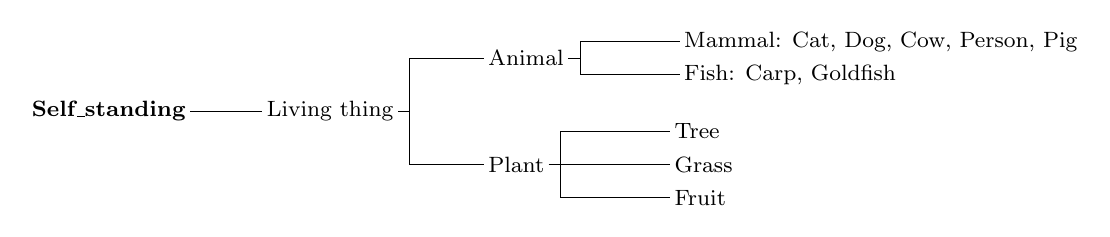
\begin{tikzpicture}[
    grow'=right, level distance=1.95cm, edge from parent path={(\tikzparentnode.east) -- ++(0.15,0) |- (\tikzchildnode.west)},
    every node/.style={font=\footnotesize, anchor=west, inner sep=1.5pt},
    level 1/.style={sibling distance=2.7cm},
    level 2/.style={sibling distance=1.35cm},
    level 3/.style={sibling distance=0.42cm}]
  \node[font=\footnotesize\bfseries] {Self\_standing}
    child {node {Living thing}
      child {node {Animal}
        child {node {Mammal: Cat, Dog, Cow, Person, Pig}}
        child {node {Fish: Carp, Goldfish}}}
      child {node {Plant}
        child {node {Tree}}
        child {node {Grass}}
        child {node {Fruit}}}};
\end{tikzpicture}

\medskip
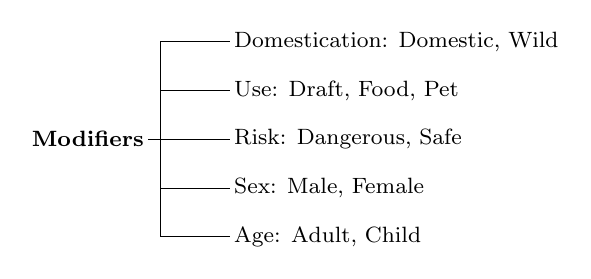
\begin{tikzpicture}[
    grow'=right, level distance=1.8cm, edge from parent path={(\tikzparentnode.east) -- ++(0.15,0) |- (\tikzchildnode.west)},
    every node/.style={font=\footnotesize, anchor=west, inner sep=1.5pt},
    level 1/.style={sibling distance=0.62cm}]
  \node[font=\footnotesize\bfseries] {Modifiers}
    child {node {Domestication: Domestic, Wild}}
    child {node {Use: Draft, Food, Pet}}
    child {node {Risk: Dangerous, Safe}}
    child {node {Sex: Male, Female}}
    child {node {Age: Adult, Child}};
\end{tikzpicture}
\hspace{0.1cm}
\begin{tabular}[b]{@{}l@{}}
\textbf{Definables}\\ Carnivore, Herbivore\\ Child, Parent\\ Mother, Father\\
Food animal, Draft animal\\[4pt]
\textbf{Relations}\\ eats, owns, parent-of, \ldots
\end{tabular}
\captionof{figure}{The animals \& plants terms reorganised: self-standing entities and
modifiers as pure trees (the primitives), plus the definables and the relations, kept
aside.}
\label{fig:animals-plants}
\end{center}

\begin{nbintuition}[why pure trees?]
\emph{Pet} looks like a subclass of \emph{Animal}, \emph{Dog} too; but a dog can be a
pet or not, and a pet can be a dog, a cat or a goldfish. If we put \emph{Pet} in the
same tree as \emph{Dog} we get multiple inheritance everywhere and the tree becomes a
tangle. Keeping ``what a thing is'' (Dog) separate from ``how it is used'' (Pet) and
``what state it is in'' (Domestic) keeps each tree simple. A class like \emph{Pet dog}
can then be \emph{defined} as Dog $\sqcap$ having use Pet, and the reasoner works out
that it is both a Dog and a Pet.
\end{nbintuition}

\textbf{Comments help to clarify}: when a class is used in a special way, add a comment,
e.g.\ on \emph{Living thing}: ``abstract ancestor concept including all living things;
restrict to plants and animals for now''.

\paragraph{Class inheritance.}
Classes are organised into \textbf{subclass--superclass} hierarchies (also called
generalisation--specialisation hierarchies). Two classes are in an ``is-a'' relation if every instance of the subclass
is an instance of the superclass. Classes can be seen as \textbf{sets}: a subclass is a
subset of its superclass. Examples: Mammal is a subclass of Animal; every penguin is a
bird (Tweety, an instance of Penguin, is also an instance of Bird); Draft animal is a
subclass of Animal.

\paragraph{Levels in the class hierarchy.}
Three modes of development:
\begin{itemize}[nosep]
  \item \textbf{top-down}: define the most general concepts first and then specialise
        them;
  \item \textbf{bottom-up}: define the most specific concepts first, then group them into
        more general classes;
  \item a \textbf{combination} (the typical choice): breadth at the top level and depth
        along a few branches to test the design.
\end{itemize}
\textbf{Class inheritance is transitive}: if A is a subclass of B and B a subclass of C,
then A is a subclass of C.

\begin{center}
\begin{tikzpicture}[w/.style={font=\small, anchor=west, inner sep=1pt}, y=0.48cm,
    br/.style={decorate, decoration={brace, amplitude=4pt}, thick}]
  \node[w] at (0,0) {Wine};
  \foreach \t/\y in {White wine/1, Rosé wine/2, Red wine/3}
     {\node[w, text=nbgreen!60!black] at (0.5,-\y) {\t}; \draw[nbgray] (0.2,-\y+0.6) |- (0.5,-\y);}
  \foreach \t/\y in {Beaujolais/4, Red Burgundy/5, Red Zinfandel/6, Red Bordeaux/7}
     {\node[w, text=nbblue] at (1.0,-\y) {\t}; \draw[nbgray] (0.7,-\y+0.6) |- (1.0,-\y);}
  \foreach \t/\y in {Médoc/8}
     {\node[w, text=nbteal] at (1.5,-\y) {\t}; \draw[nbgray] (1.2,-\y+0.6) |- (1.5,-\y);}
  \foreach \t/\y in {Pauillac/9, Margaux/10}
     {\node[w, text=nbteal] at (2.0,-\y) {\t}; \draw[nbgray] (1.7,-\y+0.6) |- (2.0,-\y);}
  \foreach \t/\y in {St.\ Émilion/11, Graves/12}
     {\node[w, text=nbteal] at (1.5,-\y) {\t}; \draw[nbgray] (1.2,-\y+0.6) |- (1.5,-\y);}
  \foreach \t/\y in {{Cabernet Franc, Cabernet Sauvignon, Pinot Noir, Chianti, \ldots}/13}
     {\node[w, text=nbblue] at (1.0,-\y) {\t}; \draw[nbgray] (0.7,-\y+0.6) |- (1.0,-\y);}
  \draw[br, nbgreen!60!black] (3.2,-0.7) -- (3.2,-3.3) node[midway, right=5pt, font=\small\bfseries] {top level};
  \draw[br, nbblue] (4.4,-3.7) -- (4.4,-7.3) node[midway, right=5pt, font=\small\bfseries] {middle level};
  \draw[br, nbteal] (4.4,-7.7) -- (4.4,-12.3) node[midway, right=5pt, font=\small\bfseries] {bottom level};
\end{tikzpicture}
\captionof{figure}{Levels in the class hierarchy of the wine ontology (redrawn and
simplified from a Protégé screenshot): general classes at the top, specific ones at the
bottom.}
\end{center}

% ---------------------------------------------------------------------------
\subsubsection{Step 6: define properties}
\slidesrc{Ontology development: 44--47}

This step is often interleaved with the previous one. \textbf{Properties} (called
\emph{roles} in description logics, \emph{slots} in frames) describe the attributes of
the members of a class.

\begin{nbfact}{properties are inherited}
The semantics of \emph{subClassOf} demands that whenever A is a subclass of B, every
property statement that holds for instances of B also applies to instances of A. So it
makes sense to attach a property to the \textbf{highest} class in the hierarchy to which
it applies (attach \emph{eats} to Animal, not separately to Cat, Dog, Cow, \ldots).
\end{nbfact}

Types of properties, on the wine example:
\begin{itemize}[nosep]
  \item \textbf{intrinsic} properties: flavour and colour of a wine (they belong to the
        thing itself);
  \item \textbf{extrinsic} properties: name and price of a wine (assigned from outside);
  \item \textbf{parts}: the ingredients of a dish;
  \item \textbf{relations to other objects}: the producer of a wine (a winery).
\end{itemize}
They are represented by two kinds of properties (Section~\ref{sec:ontology-languages}):
\begin{itemize}[nosep]
  \item \textbf{datatype properties}: simple values (strings, numbers): name, price;
  \item \textbf{object properties}: complex values, other objects: the producer is an
        instance of Winery.
\end{itemize}
In the animals example, the modifiers of Figure~\ref{fig:animals-plants} (domestication,
use, risk, sex, age) and the relations (eats, owns, parent-of) become properties.

% ---------------------------------------------------------------------------
\subsubsection{Step 7: define constraints}
\slidesrc{Ontology development: 48--56}

\paragraph{Domain and range.}
For each property, state the \textbf{domain} (the class of the things that can have it)
and the \textbf{range} (the class of its values):
\begin{center}
\small
\begin{tabularx}{\linewidth}{@{}>{\raggedright\arraybackslash}X l l l@{}}
\toprule
\textbf{statement} & \textbf{property} & \textbf{domain} & \textbf{range} \\
\midrule
Animal eats Living\_thing & eats & Animal & Living\_thing \\
Person owns Living\_thing except person & owns & Person & Living\_thing $\sqcap \neg$Person \\
Living\_thing parent\_of Living\_thing & parent\_of & Living\_thing & Living\_thing \\
\bottomrule
\end{tabularx}
\end{center}
If anything is used in a special way, add a text comment. E.g.\ on \emph{eats}:
``ignore the difference between parts of living things and living things; also things
derived from living things'' (strictly, a cow eats \emph{leaves}, not whole plants, and
we eat cheese, which is not a living thing).

\paragraph{Definable things.}
Paraphrase the definitions and formalise them in terms of the primitives, the relations
and other definables. Note any assumptions (as comments when implementing).

\begin{nbexample}{three definitions}
The slides write them in the Manchester syntax used by Protégé (\emph{and}, \emph{some},
\emph{only}); next to it the same in description-logic notation, where $\sqcap$ is
``and'', $\exists r.C$ is ``has some $r$-value in $C$'' and $\forall r.C$ is ``all
$r$-values are in $C$'':
\begin{center}
\small
\begin{tabularx}{\linewidth}{@{}>{\raggedright\arraybackslash}X l@{}}
\toprule
\textbf{in words} & \textbf{formal} \\
\midrule
A \emph{Parent} is an animal that is the parent of some other animal (ignore plants for
  now) & Parent $\equiv$ Animal $\sqcap\ \exists$parent\_of.Animal \\
A \emph{Herbivore} is an animal that eats only plants & Herbivore $\equiv$ Animal
  $\sqcap\ \forall$eats.Plant \\
An \emph{Omnivore} is an animal that eats both plants and animals & Omnivore $\equiv$
  Animal $\sqcap\ \exists$eats.Animal $\sqcap\ \exists$eats.Plant \\
\bottomrule
\end{tabularx}
\end{center}
\end{nbexample}

\begin{nbwarning}[``only'' does not mean ``some'']
$\forall$eats.Plant (``eats \emph{only} plants'') is also true of something that eats
\emph{nothing}: all the (zero) things it eats are plants. That is why the slides add
``NB: all animals eat some living thing'': with that axiom, an animal that eats only
plants really eats some plant. Mixing up \emph{some} ($\exists$) and \emph{only}
($\forall$) is the most common modelling error in OWL.
\end{nbwarning}

\paragraph{Fill in properties at the class level.}
What can we say about \emph{all} members of a class? All cows eat some plants; all cats
eat some animals; all pigs eat some animals and eat some plants. In Protégé this can be
done with a ``property matrix'' (one row per class, one column per property: Cat eats
Animal, Dog eats Animal, Cow eats Grass and Leafy\_plant, Person eats Animal and Plant).

\paragraph{Check with the classifier: the closure axiom.}
A \textbf{classifier} (reasoner) computes the hierarchy of the defined classes. We expect
\emph{Cow} to be classified as a \emph{Herbivore}. It is not. Why?

\begin{nbexample}{why cows are not herbivores (yet)}
What we have said: cows are animals and, among other things, eat some grass and eat some
leafy plants:
\[
  \text{Cow} \sqsubseteq \text{Mammal} \sqcap \exists\text{eats.Grass} \sqcap
  \exists\text{eats.Leafy\_plant}.
\]
Nothing here says that cows eat \emph{only} plants: a cow could also eat some animal,
and the reasoner must allow that. What we need to say: cows eat some plants
\textbf{and eat only plants}. We add the \textbf{closure axiom}
\[
  \text{Cow} \sqsubseteq \forall\text{eats.}(\text{Grass} \sqcup \text{Leafy\_plant}),
\]
which ``closes'' the list of things cows eat. Now every cow is an Animal that eats only
plants, so the reasoner classifies Cow under Herbivore.
\end{nbexample}

\begin{nbdef}{Open vs.\ closed world reasoning}
\begin{itemize}[nosep]
  \item \textbf{Open world} reasoning: \emph{negation as contradiction}. Anything might
        be true unless it can be proven false. We reason about \emph{any} world
        consistent with what we know.
  \item \textbf{Closed world} reasoning: \emph{negation as failure}. Anything that cannot
        be found is false. We reason about \emph{this} world, the one in the database.
\end{itemize}
OWL ontologies use the open world assumption: \textbf{ontologies are not databases}
(Section~\ref{sec:what-is-an-ontology}).
\end{nbdef}

\begin{nbintuition}[the closure axiom and the open world]
In a database, if the table of what cows eat lists only grass and leafy plants, then cows
eat nothing else: missing rows are false (closed world). In an ontology, missing
information is just \emph{unknown} (open world): ``cows eat grass'' leaves open that they
also eat fish. The closure axiom is how we tell an open-world reasoner ``and that is
all''.
\end{nbintuition}

% ---------------------------------------------------------------------------
\subsubsection{Step 8: create instances}
\slidesrc{Ontology development: 57--60}

To create an instance of a class: the class becomes the \textbf{direct type} of the
instance, and every superclass of the direct type is also a type of the instance (Tweety
is a Penguin, hence a Bird, hence an Animal). Then assign the slot (property) values;
they must conform to the facet constraints, and knowledge-acquisition tools often check
this.

Filling the ontology with instances is a \textbf{separate step}, and the number of
instances is much larger than the number of classes. So \textbf{populating} an ontology
is usually not done by hand: instances are retrieved from legacy data sources
(databases) or \textbf{extracted automatically from a text corpus}: this is
\emph{ontology population}, part of ontology learning (Section~\ref{sec:ontology-learning}).

\begin{nbsummary}[the design process]
\begin{itemize}[nosep]
  \item Many methodologies (On-To-Knowledge, HCOME, DILIGENT, NeOn, DOGMA, RapidOWL,
        \ldots); the lecturer's choice: Noy \& McGuinness, \emph{Ontology Development
        101}.
  \item Cycle of 8 steps: requirement and domain analysis $\to$ scope $\to$ reuse $\to$
        enumerate terms $\to$ classes $\to$ properties $\to$ constraints $\to$
        instances, and again.
  \item Competency questions define the scope and test the ontology.
  \item Reuse: libraries, upper ontologies (SUO, Cyc), general (WordNet), domain (GO,
        UMLS).
  \item Terms: nouns $\to$ classes, verbs $\to$ properties; card sorting.
  \item Classes: self-standing entities and modifiers as pure trees (primitives);
        definables defined by axioms; inheritance is transitive; top-down, bottom-up or
        combined.
  \item Properties: intrinsic, extrinsic, parts, relations; datatype vs.\ object; attach
        to the highest class.
  \item Constraints: domain and range; definitions with \emph{some} ($\exists$) and
        \emph{only} ($\forall$); closure axioms; open world (ontology) vs.\ closed world
        (database).
  \item Instances: many, populated automatically from databases or text.
\end{itemize}
\end{nbsummary}

\subsection{N-ary Relations}
\label{sec:n-ary-relations}
\slidesrc{Ontology development: 61--73}

\subsubsection{The problem}
\slidesrc{Ontology development: 61--62}

In OWL (and RDF) a property is a \textbf{binary} relation: an instance of a property
links two individuals (\emph{Christine} --has\_diagnosis$\to$ \emph{Breast\_Tumor}), or
an individual and a value. Sometimes, though, the most natural way to describe a
situation links an individual to \emph{more than one} other individual or value. Such
relations are called \textbf{n-ary relations}. Three issues arise:
\begin{enumerate}[nosep]
  \item how do we describe \emph{an instance of a relation} (e.g.\ attach a probability
        to a diagnosis)?
  \item how do we represent relations among more than two individuals?
        $\Rightarrow$ \textbf{Pattern 1};
  \item how do we represent a relation in which one participant is an \emph{ordered
        list} of individuals? $\Rightarrow$ \textbf{Pattern 2}.
\end{enumerate}
The solutions come from the W3C Working Group Note \emph{Defining N-ary Relations on the
Semantic Web} (W3C Semantic Web Best Practices and Deployment Working Group).

\begin{nbexample}{four situations that binary properties cannot express}
\begin{enumerate}[nosep]
  \item \emph{Christine has breast tumor with high probability}: a relation first thought
        to be binary needs a further argument (the probability).
  \item \emph{Steve has temperature, which is high, but falling}: two binary properties
        always go together and should be represented as one n-ary relation.
  \item \emph{John buys a ``Lenny the Lion'' book from books.example.com for \$15 as a
        birthday gift}: from the beginning, the relation is among several things.
  \item \emph{United Airlines flight 3177 visits the following airports: LAX, DFW, and
        JFK}: one argument is fundamentally a \emph{sequence}, not a single individual.
\end{enumerate}
\end{nbexample}

\subsubsection{Pattern 1: the relation becomes a class}
\slidesrc{Ontology development: 63--70}

\begin{nbfact}{Pattern 1 (reification)}
Represent the relation as a \textbf{class} rather than a property. Each individual
instance of this class corresponds to one instance of the relation; additional
properties provide binary links to each argument of the relation. The classes created in
this way are often called \textbf{reified relations} (to \emph{reify} = to make a thing
out of something abstract).
\end{nbfact}

\paragraph{Case 1: additional attributes describing a relation.}
\emph{Christine has breast tumor with high probability.} We create an individual that
represents the relation instance itself, with a link from the subject (Christine) to it,
and links from it to everything else (the diagnosis and its probability).

\begin{center}
\begin{tikzpicture}[ind/.style={draw, fill=black!5, font=\small, inner sep=3pt},
    rel/.style={draw=nborange, fill=nborange!25, font=\small, inner sep=3pt},
    l/.style={font=\scriptsize, midway, fill=white, inner sep=1pt}, ->, >=Stealth]
  \node[ind] (c) {Christine};
  \node[rel, right=2.2cm of c] (d) {\_:Diagnosis\_Relation\_1};
  \node[ind, anchor=west] (t) at ($(d.east)+(2.2,0.9)$) {Breast\_Tumor\_Christine};
  \node[ind, anchor=west] (h) at ($(d.east)+(2.2,-0.9)$) {HIGH};
  \draw (c) -- node[l] {has\_diagnosis} (d);
  \draw (d) -- node[l] {diagnosis\_value} (t);
  \draw (d) -- node[l] {diagnosis\_probability} (h);
\end{tikzpicture}
\captionof{figure}{Pattern 1, case 1: the diagnosis relation becomes an individual.}
\end{center}

The individual \texttt{\_:Diagnosis\_Relation\_1} is a single object that encapsulates
both the diagnosis and its probability: it contains all the information of the three
original arguments (who is diagnosed, what the diagnosis is, how probable it is). In RDF
such instances are \textbf{blank nodes}: an \texttt{rdf:Description} element without an
\texttt{rdf:about} attribute, i.e.\ a node without a global name (hence the
``\texttt{\_:}'' prefix). Class definitions: Person --has\_diagnosis$\to$
Diagnosis\_Relation (all values from); Diagnosis\_Relation --diagnosis\_value$\to$ Disease
and --diagnosis\_probability$\to$ Probability (both functional: exactly one value).

\paragraph{Case 2: different aspects of the same relation.}
\emph{Steve has temperature, which is high, but falling.} This is not a binary relation
with an extra attribute: it relates the individual Steve to a \emph{complex object}
representing different facts about his temperature.

\begin{center}
\begin{tikzpicture}[ind/.style={draw, fill=black!5, font=\small, inner sep=3pt},
    rel/.style={draw=nborange, fill=nborange!25, font=\small, inner sep=3pt},
    l/.style={font=\scriptsize, midway, fill=white, inner sep=1pt}, ->, >=Stealth]
  \node[ind] (s) {Steve};
  \node[rel, right=2.6cm of s] (o) {\_:Temperature\_Observation\_1};
  \node[ind, anchor=west] (e) at ($(o.east)+(2.6,0.9)$) {ELEVATED};
  \node[ind, anchor=west] (f) at ($(o.east)+(2.6,-0.9)$) {FALLING};
  \draw (s) -- node[l] {has\_temperature} (o);
  \draw (o) -- node[l] {temperature\_value} (e);
  \draw (o) -- node[l] {temperature\_trend} (f);
\end{tikzpicture}
\captionof{figure}{Pattern 1, case 2: an observation object groups two aspects of
Steve's temperature.}
\end{center}

Such cases often appear while an ontology \textbf{evolves}, when one realises that two
relations must be collapsed into one: initially one might have had two properties,
\emph{has\_temperature\_level} and \emph{has\_temperature\_trend}, both relating to
people; then one realises they are inextricably intertwined, because one needs to talk
about ``temperatures that are elevated but falling''.

\paragraph{Case 3: n-ary relation with no distinguished participant.}
\emph{John buys a ``Lenny the Lion'' book from books.example.com for \$15 as a birthday
gift.} The relation links individuals that play different roles, and none of them stands
out as the ``owner'' of the relation. We create an individual for the relation instance
with links to \emph{all} participants.

\begin{center}
\begin{tikzpicture}[ind/.style={draw, fill=black!5, font=\small, inner sep=3pt},
    rel/.style={draw=nborange, fill=nborange!25, font=\small, inner sep=3pt},
    l/.style={font=\scriptsize, midway, fill=white, inner sep=1pt}, ->, >=Stealth]
  \node[rel] (p) at (0,0) {Purchase\_1};
  \node[ind] (j) at (-6.0,-1.0) {John};
  \node[ind] (b) at (-4.2,-3.0) {books.example.com};
  \node[ind] (l) at (0,-3.0) {Lenny\_The\_Lion};
  \node[ind] (m) at (4.0,-3.0) {Birthday\_Gift};
  \node[ind] (d) at (6.0,-1.0) {\$15};
  \draw (p) -- node[l] {has\_buyer} (j);
  \draw (p) -- node[l] {has\_seller} (b);
  \draw (p) -- node[l] {has\_object} (l);
  \draw (p) -- node[l] {has\_purpose} (m);
  \draw (p) -- node[l] {has\_amount} (d);
\end{tikzpicture}
\captionof{figure}{Pattern 1, case 3: a Purchase individual linked to all participants.
Class level: Purchase --has\_buyer$\to$ Person, --has\_seller$\to$ Company,
--has\_object$\to$ Object, --has\_purpose$\to$ Purpose, --has\_amount$\to$ Quantity.}
\end{center}

\begin{nbwarning}[considerations in introducing a new class]
\begin{itemize}[nosep]
  \item The individuals that represent relation instances (and often their classes) are
        not given meaningful names, just labels: they do not stand on their own, they
        only group other objects together, so a distinguishing name serves no purpose
        (the same is done when reifying statements in RDF).
  \item Creating a class to represent an n-ary relation \textbf{limits the use of many
        OWL constructs} and creates a \textbf{maintenance problem}, especially with
        inverse relations (the inverse of a 5-ary relation is not a single property).
\end{itemize}
\end{nbwarning}

\subsubsection{Pattern 2: lists for arguments in a relation}
\slidesrc{Ontology development: 71--73}

Some n-ary relations do not fall into the cases above: they are more like a list or
sequence of arguments. \emph{United Airlines flight 3177 visits the following airports:
LAX, DFW, and JFK}: the relation holds between the flight and the airports, \emph{in the
order} in which the aircraft arrives at each one. It might hold between any number of
arguments, there is no natural way to break it into distinct properties (first\_stop,
second\_stop, \ldots), and the order is highly meaningful.

\begin{nbfact}{Pattern 2}
When all participants but one have no specific role and form an ordered list, connect
them into a \textbf{sequence} with an ordering relation, and relate the one remaining
participant to the sequence (or to its first element).
\end{nbfact}

\begin{center}
\begin{tikzpicture}[ind/.style={draw, fill=black!5, font=\small, inner sep=3pt},
    rel/.style={draw=nborange, fill=nborange!25, font=\small, inner sep=3pt},
    l/.style={font=\scriptsize, midway, fill=white, inner sep=1pt}, ->, >=Stealth]
  \node[ind] (f) at (-0.6,0) {UA\_1377};
  \node[rel] (s1) at (4,0) {UA\_1377\_1};
  \node[rel] (s2) at (4,-1.6) {UA\_1377\_2};
  \node[rel] (s3) at (4,-3.2) {UA\_1377\_3};
  \node[ind] (a1) at (8,0) {LAX};
  \node[ind] (a2) at (8,-1.6) {DFW};
  \node[ind] (a3) at (8,-3.2) {JFK};
  \draw (f) -- node[l] {flight\_sequence} (s1);
  \draw (s1) -- node[l] {next\_segment} (s2);
  \draw (s2) -- node[l] {next\_segment} (s3);
  \draw (s1) -- node[l] {destination} (a1);
  \draw (s2) -- node[l] {destination} (a2);
  \draw (s3) -- node[l] {destination} (a3);
\end{tikzpicture}
\captionof{figure}{Pattern 2: the flight points to its first segment; segments are
chained by \emph{next\_segment}; each segment has a destination.}
\end{center}

\emph{nextSegment} is an ordering relation between instances of the class
\emph{FlightSegment}; each segment has a property for its destination. A special
subclass, \emph{FinalFlightSegment}, has a \textbf{maximum cardinality of 0} on
\emph{nextSegment}: the last segment has no next one, which marks the end of the
sequence. (This is how linked lists work in programming: each node points to the next,
the last points to nothing.)

\begin{nbsummary}[n-ary relations]
\begin{itemize}[nosep]
  \item OWL properties are binary; n-ary relations need a pattern.
  \item Pattern 1 (reified relation): a new class whose instances are the relation
        instances, with one binary property per argument. Case 1: extra attributes of a
        relation (diagnosis + probability); case 2: different aspects of one relation
        (temperature value + trend); case 3: no distinguished participant (purchase).
        Instances are often blank nodes; drawbacks: fewer OWL constructs usable,
        maintenance problems with inverses.
  \item Pattern 2: ordered arguments as a linked sequence (flight segments with
        \emph{nextSegment}; final segment with max cardinality 0).
\end{itemize}
\end{nbsummary}

\subsection{Ontology Learning}
\label{sec:ontology-learning}
\slidesrc{Ontology learning: 1--25; Ontology development: 74}

Building an ontology by hand (Section~\ref{sec:design-process}) is slow and expensive.
\textbf{Ontology learning} uses NLP and machine learning to do part of the work
automatically. The deck is a tutorial by Ícaro Medeiros (CIn--UFPE, 2008).

\subsubsection{What, why and from where}
\slidesrc{Ontology learning: 4--9}

The field has \textbf{too many names for the same subject}: ontology extraction,
emergence, generation, acquisition, discovery, population, enrichment\ldots\ The common
name, after Philipp Cimiano's book \emph{Ontology Learning and Population from Text}
(2006), is \textbf{ontology learning} (OL).

\begin{nbdef}{Ontology learning}
\textbf{Ontology learning} is the set of methods and techniques for
\begin{itemize}[nosep]
  \item building an ontology from scratch;
  \item enriching or adapting an existing ontology;
\end{itemize}
by extracting concepts and relations (from text or other sources) to form an ontology.
OL is a \textbf{semi-automatic} task of information extraction: a human remains in the
loop to validate and correct.
\end{nbdef}

\paragraph{Why?}
Ontology engineering has three problems (Maedche and Staab, 2001):
\begin{itemize}[nosep]
  \item \textbf{time}: can you develop an ontology fast?
  \item \textbf{difficulty}: is it difficult to build an ontology?
  \item \textbf{confidence}: how do you know that you have got the ontology right?
\end{itemize}
OL can help with all three, especially with the \textbf{knowledge acquisition
bottleneck}: experts are few and busy, and writing their knowledge down by hand is the
slowest part of building any knowledge-based system.

\paragraph{Information sources.}
Relevant text (mainly Web documents); Web document schemata (XML, DTD, RDF); databases
on the Web; dictionaries; semi-structured documents; personal wikis, e-mail and file
folders; existing Web ontologies.

\begin{center}
\begin{tikzpicture}[st/.style={draw=nborange, fill=nborange!10, font=\small,
    rounded corners=2pt, inner sep=4pt}, arr/.style={-{Stealth}, very thick, nbteal}]
  \draw[line width=14pt, black!12] (0,0) circle (2.6);
  \node[font=\scriptsize\itshape] at (0,2.6) {Legacy + Application Data};
  \node[font=\scriptsize\itshape] at (0,-2.6) {Legacy + Application Data};
  \node[draw, circle, fill=nbteal!10, font=\scriptsize, align=center, minimum size=1.7cm]
       at (0,0) {Domain\\ Ontology};
  \draw[arr] (150:1.6) arc (150:30:1.6);
  \draw[arr] (-30:1.6) arc (-30:-150:1.6);
  \node[font=\scriptsize\itshape, text=nbteal] at (0,1.25) {ontology learning};
  \node[font=\scriptsize\itshape, text=nbteal] at (0,-1.25) {ontology learning};
  \node[st] at (150:2.6) {Extract};
  \node[st] at (40:2.6) {Prune};
  \node[st] at (-20:2.6) {Refine};
  \node[st] at (-60:2.6) {Apply};
  \node[st] at (210:2.6) {Import / Reuse};
\end{tikzpicture}
\captionof{figure}{The ontology engineering cycle of Maedche and Staab (2001), redrawn:
import/reuse existing ontologies, extract, prune, refine, apply, and start again.
Ontology learning is not only the task of extraction.}
\end{center}

The cycle shows that OL is \textbf{not only extraction}: one also \emph{imports} and
reuses existing ontologies, \emph{prunes} what is irrelevant for the application,
\emph{refines} the result, and \emph{applies} it, which produces new data for the next
round.

\subsubsection{How to learn ontologies}
\slidesrc{Ontology learning: 10--15}

The main families of techniques: natural language processing; dictionary parsing;
statistical analysis; machine learning; hierarchical concept clustering; Formal Concept
Analysis (lattices).

\paragraph{Why text?}
Text is massively available on the Web; relevant texts contain relevant knowledge about a
domain; and when an ontology is learnt from text, the \emph{linguistic} knowledge (how
concepts are named and talked about) remains associated with the ontology (Sintek et
al., 2004).

\begin{nbintuition}[OL as reverse engineering (Buitelaar et al., 2005)]
People share a model of the world (a ``shared world model'') and use it to
\emph{write} texts: newspapers, manuals, Web pages. Ontology learning goes the opposite
way: from the texts back to the model. It is \textbf{reverse engineering}: like
recovering the design of a program from its compiled code, we recover the conceptual
model from the documents it produced. And like reverse engineering, it is only partial:
much of the shared knowledge is never written down because everybody already knows it.
\end{nbintuition}

\begin{center}
\begin{tikzpicture}[lay/.style={draw, fill=nbblue!6, font=\small, minimum height=0.75cm,
    anchor=east}]
  \foreach \t/\w/\y/\ex in {
      Terms/6.1/0/{disease, illness, hospital},
      (Multilingual) Synonyms/5.8/0.75/{\{disease, illness, Krankheit\}},
      Concepts/5.5/1.5/{DISEASE := $\langle$Int, Ext, Lex$\rangle$},
      Taxonomy/5.2/2.25/{is\_a(DOCTOR, PERSON)},
      Relations/4.9/3.0/{cure(dom: DOCTOR, range: DISEASE)},
      Rules \& Axioms/4.6/3.75/{$\forall x, y\,(\mathit{sufferFrom}(x,y) \to \mathit{ill}(x))$}}
  {
    \node[lay, minimum width=\w cm - 1.6cm] at (12,\y) {\t};
    \node[font=\small\itshape, anchor=east] at ({12-(\w-1.6)-0.15},\y) {\ex};
  }
\end{tikzpicture}
\captionof{figure}{The ontology learning layer cake (Buitelaar et al., 2005), redrawn.
Each layer is a learning task that builds on the layers below it; on the left, an
example of the output of each task.}
\label{fig:layer-cake}
\end{center}

\begin{nbfact}{the layer cake}
Ontology learning from text is organised in six layers, from the bottom:
\begin{enumerate}[nosep]
  \item \textbf{terms}: the relevant words and phrases of the domain (\emph{disease},
        \emph{illness}, \emph{hospital});
  \item \textbf{(multilingual) synonyms}: groups of terms with the same meaning, also
        across languages (\emph{disease}, \emph{illness}, German \emph{Krankheit});
  \item \textbf{concepts}: a concept is defined by its \textbf{int}ension, its
        \textbf{ext}ension and its \textbf{lex}ical realisations (see below);
  \item \textbf{taxonomy}: the is-a hierarchy between concepts (a doctor is a person);
  \item \textbf{relations}: other relations between concepts, with domain and range
        (doctors cure diseases);
  \item \textbf{rules and axioms}: general logical statements (whoever suffers from
        something is ill).
\end{enumerate}
Lower layers are easier to learn automatically and more reliable; upper layers are
harder and need more human validation.
\end{nbfact}

\subsubsection{Term extraction}
\slidesrc{Ontology learning: 16--18}

\textbf{Linguistic methods} reuse the syntactic tools of the course:
\begin{itemize}[nosep]
  \item \textbf{part-of-speech tagging} (Section~\ref{sec:pos-tagging}) to identify the
        syntactic class: a noun suggests a class, a verb a relation;
  \item \textbf{stemming} (Section~\ref{sec:stemming-lemmatization}): \emph{formalize},
        \emph{formalization}, \emph{formalized}, \emph{formalizing} are one term;
  \item \textbf{head-modifier analysis}: in \emph{fast car} the head is \emph{car} and
        \emph{fast} a modifier; in \emph{the hood of the car}, \emph{hood} is a part of
        \emph{car};
  \item \textbf{grammatical function analysis}: ``John played football in the garden''
        $\to$ \emph{play(John, football)}: the subject and the object of a verb become
        the arguments of a relation.
\end{itemize}

\textbf{Statistical methods}:
\begin{itemize}[nosep]
  \item \textbf{term weighting} with TF-IDF (Section~\ref{sec:stop-words-tfidf});
  \item \textbf{co-occurrence analysis} (a common method in text mining);
  \item \textbf{comparison of frequencies between a domain corpus and a general corpus}:
        a word much more frequent in medical texts than in newspapers (\emph{tumour}) is
        likely a medical term; a word equally frequent in both (\emph{table}) is not.
\end{itemize}

\textbf{Hybrid methods}: linguistic rules extract term candidates (e.g.\ the POS pattern
``adjective* noun+'' finds \emph{heart disease}, \emph{chronic kidney disease}), then
statistics filter them (before or after).

\subsubsection{Synonym extraction}
\slidesrc{Ontology learning: 19--20}

Two approaches: \textbf{extending WordNet} (\emph{term classification}: attach a new
term to the right synset of WordNet, Section~\ref{sec:wordnet}) and
\textbf{co-occurrence between terms} (\emph{term clustering}: terms with similar
contexts are grouped together, the distributional hypothesis of
Section~\ref{sec:distributional-hypothesis}).

\subsubsection{Concept extraction}
\slidesrc{Ontology learning: 21--25}

A term may indicate a concept, if we define its:
\begin{itemize}[nosep]
  \item \textbf{intension}: an (in)formal definition of the objects the concept
        describes. E.g.\ ``a disease is an impairment of health or a condition of
        abnormal functioning'';
  \item \textbf{extension}: the set of objects described by the concept. E.g.\ cancer,
        heart disease;
  \item \textbf{lexical realisations}: the term itself and its (multilingual)
        synonyms.
\end{itemize}

\begin{nbintuition}[intension vs.\ extension]
The \emph{intension} is the \emph{recipe} (``what it takes to be a disease''); the
\emph{extension} is the \emph{list} (``all the diseases''). The concept ``even number
between 1 and 9'' has intension ``divisible by 2, between 1 and 9'' and extension
$\{2, 4, 6, 8\}$. In an ontology, the class definition is the intension, and the
instances are the extension.
\end{nbintuition}

\paragraph{Learning the intension.}
An \emph{informal} definition is a shallow definition as used in WordNet (a gloss):
find the appropriate WordNet concept for a term and the appropriate conceptual relations
(Navigli and Velardi, 2004). A \emph{formal} definition gives formal constraints for
class membership, e.g.\ with Formal Concept Analysis.

\paragraph{Learning the extension: ontology population.}
Extracting the instances of a concept from text is \textbf{ontology population}. It is
related to knowledge markup and tag suggestion (semantic metadata), and it uses
\textbf{named entity recognition} (Section~\ref{sec:named-entity-recognition}):
``John is a football player'' $\to$ \emph{John} (a Person) is an instance of
\emph{Football Player}. Instances can be
\begin{itemize}[nosep]
  \item names for objects: persons, organisations, countries, cities;
  \item event instances: a football match, with its teams, players, officials, \ldots
\end{itemize}

\begin{nbwarning}[what the shortened deck leaves out]
The outline of the tutorial continues with taxonomy, relation and axiom learning,
ontology learning from folksonomies (collaborative tags), tools and conclusions. These
parts are not in the shortened deck shown in class; the layer cake of
Figure~\ref{fig:layer-cake} gives what these tasks produce.
\end{nbwarning}

\begin{nbsummary}[ontology learning]
\begin{itemize}[nosep]
  \item OL (a.k.a.\ extraction, generation, acquisition, population, enrichment):
        semi-automatic building or enrichment of ontologies; fights the knowledge
        acquisition bottleneck (time, difficulty, confidence).
  \item Sources: Web text, schemata, databases, dictionaries, semi-structured documents,
        existing ontologies. OE cycle: import/reuse, extract, prune, refine, apply.
  \item Methods: NLP, dictionary parsing, statistics, ML, clustering, Formal Concept
        Analysis. OL from text = reverse engineering of the shared world model.
  \item Layer cake: terms $\to$ synonyms $\to$ concepts $\to$ taxonomy $\to$ relations
        $\to$ rules \& axioms.
  \item Terms: POS, stemming, head-modifier, grammatical functions; TF-IDF,
        co-occurrence, domain vs.\ general corpus; hybrid.
  \item Concept = intension + extension + lexical realisations; extension learning =
        ontology population, with NER.
\end{itemize}
\end{nbsummary}

\subsection{Ontology Matching}
\label{sec:ontology-matching}
\slidesrc{Ontology matching: 1--14; Ontology matching (long version): 1--112; Ontology
development: 75--76}

Different people build different ontologies of the same domain: they use different
names (\emph{PC} vs.\ \emph{Personal Computers}), different structures, different
languages. To make two systems that use two ontologies work together we must find
which entity of one corresponds to which entity of the other. This is
\textbf{ontology matching}. The source is the tutorial by Pavel Shvaiko and Jérôme
Euzenat (SWAP 2006); the slides shown in class are the definitions of correspondence and
alignment, the matching process and the application domains; the rest comes from the
long version.

\subsubsection{The matching problem}
\slidesrc{Ontology matching (long version): 2--25}

The goals of the tutorial: illustrate the role of ontology matching, give an overview of
the basic matching techniques, show how state-of-the-art systems use them, and motivate
future research.

\begin{nbdef}{Matching operation}
The \textbf{matching} operation takes as input ontologies, each consisting of a set of
discrete entities (tables, XML elements, classes, properties, \ldots), and determines as
output the \textbf{relationships} (equivalence, subsumption, \ldots) holding between
these entities.
\end{nbdef}

\begin{center}
\begin{tikzpicture}[n/.style={draw, rounded corners=2pt, font=\small, inner sep=2.5pt},
    a/.style={font=\small, text=nbgreen!60!black},
    c/.style={{Stealth}-{Stealth}, thick, nbblue},
    r/.style={font=\small, fill=white, inner sep=1pt}]
  % left schema
  \node[n, anchor=west] (e1)  at (0,0)     {Electronics};
  \node[n, anchor=west] (pc1) at (0.4,-0.8) {Personal Computers};
  \node[n, anchor=west] (mp1) at (0.8,-1.6) {Microprocessors};
  \node[a, anchor=west]       at (1.2,-2.3) {PID, Name, Quantity, Price};
  \node[n, anchor=west] (ac1) at (0.4,-3.0) {Accessories};
  \node[n, anchor=west] (ph1) at (0.4,-3.8) {Photo and Cameras};
  \node[a, anchor=west]       at (0.8,-4.5) {PID, Name, Quantity, Price};
  % right schema
  \node[n, anchor=east] (e2)  at (13,0)     {Electronics};
  \node[n, anchor=east] (pc2) at (12.6,-0.8) {PC};
  \node[n, anchor=east] (mp2) at (12.2,-1.6) {PC board};
  \node[a, anchor=east]       at (11.8,-2.3) {ID, Brand, Amount, Price};
  \node[n, anchor=east] (cp2) at (12.6,-3.0) {Cameras and Photo};
  \node[n, anchor=east] (ac2) at (12.2,-3.8) {Accessories};
  \node[n, anchor=east] (dc2) at (12.2,-4.6) {Digital Cameras};
  \node[a, anchor=east]       at (11.8,-5.3) {ID, Brand, Amount, Price};
  \draw[c] (e1) -- node[r] {$=$} (e2);
  \draw[c] (pc1) -- node[r] {$=$} (pc2);
  \draw[c] (mp1) -- node[r] {$\perp$} (mp2);
  \draw[c] (ph1.east) -- node[r, pos=0.5] {$=$} (cp2.west);
  \draw[c] (ph1.east) -- node[r, pos=0.6] {$\ge$} (dc2.west);
\end{tikzpicture}
\captionof{figure}{Motivation: two XML schemas of an electronics catalogue (redrawn,
simplified). Blue arrows are correspondences: equal ($=$), more general ($\ge$),
disjoint ($\perp$). Among the attributes (green): Name $\ge$ Brand, Quantity $=$
Amount, Price $=$ Price.}
\label{fig:xml-schemas}
\end{center}

\begin{nbexample}{reading Figure~\ref{fig:xml-schemas}}
\emph{Personal Computers} on the left is the same as \emph{PC} on the right (equivalence,
found e.g.\ by expanding the abbreviation). \emph{Microprocessors} and \emph{PC board}
are disjoint: nothing is both. \emph{Photo and Cameras} is more general than
\emph{Digital Cameras}. Among the attributes, \emph{Quantity} = \emph{Amount}
(synonyms), and \emph{Name} is more general than \emph{Brand} (a brand is a kind of
name). The second motivating example in the slides does the same with two
\emph{ontologies} of products and books (\emph{Product} vs.\ \emph{Monograph},
\emph{creator} vs.\ \emph{author}, \emph{Person} vs.\ \emph{Human}), including
instances such as ``Bertrand Russell: My life'' (an Autobiography) and ``Albert Camus:
La chute'' (Literature).
\end{nbexample}

\paragraph{Schema matching vs.\ ontology matching.}
\textbf{Differences}: schemas often do not give explicit semantics for their data;
relational schemas provide no generalisation (no is-a); ontologies are logical systems
that constrain the meaning, defined as sets of logical axioms. \textbf{Commonalities}:
both provide a vocabulary of terms that describes a domain of interest, and both
constrain the meaning of these terms. Techniques developed for both problems are of
mutual benefit.

\paragraph{Scope.}
Heterogeneity between ontologies can occur when different \emph{languages} are used
(OWL vs.\ XML schema), different \emph{terminologies} (\emph{car} vs.\
\emph{automobile}), different \emph{modelling} (colour as a property vs.\ as a class),
\ldots\ Reducing heterogeneity takes two steps: \textbf{match}, which determines the
alignment, and \textbf{process the alignment} (merging, transforming, \ldots). Matching
can happen at \textbf{design time} (by the developers, before the system runs) or at
\textbf{run time} (on the fly, e.g.\ when two agents meet for the first time).

\subsubsection{Correspondence, alignment, matching process}
\slidesrc{Ontology matching: 1--13; Ontology matching (long version): 26--38}

\begin{nbdef}{Correspondence}
Given two ontologies $O$ and $O'$, a \textbf{correspondence} $M$ between $O$ and $O'$ is
a 5-tuple $\langle id, e, e', R, n\rangle$ such that:
\begin{itemize}[nosep]
  \item $id$ is a unique \textbf{identifier} of the correspondence;
  \item $e$ and $e'$ are \textbf{entities} of $O$ and $O'$ (e.g.\ XML elements, classes);
  \item $R$ is a \textbf{relation}, e.g.\ equivalence ($=$), more general
        ($\sqsupseteq$), disjointness ($\perp$);
  \item $n$ is a \textbf{confidence measure} in some mathematical structure (typically
        in the $[0,1]$ range).
\end{itemize}
\end{nbdef}

\begin{nbdef}{Alignment}
Given two ontologies $O$ and $O'$, an \textbf{alignment} $A$ between $O$ and $O'$
\begin{itemize}[nosep]
  \item is a \textbf{set of correspondences} on $O$ and $O'$;
  \item with some \textbf{cardinality}: 1-1, 1-*, etc.;
  \item with some additional \textbf{metadata} (method, date, properties, etc.).
\end{itemize}
\end{nbdef}

\begin{nbexample}{correspondences from Figure~\ref{fig:xml-schemas}}
\begin{align*}
  &\langle c_1,\ \text{Personal Computers},\ \text{PC},\ =,\ 0.95\rangle\\
  &\langle c_2,\ \text{Microprocessors},\ \text{PC board},\ \perp,\ 0.80\rangle\\
  &\langle c_3,\ \text{Photo and Cameras},\ \text{Digital Cameras},\ \sqsupseteq,\ 0.70\rangle
\end{align*}
The set $\{c_1, c_2, c_3, \ldots\}$ is an alignment. A \textbf{1-1} alignment matches each
entity to at most one entity of the other ontology; a \textbf{1-*} alignment lets one
entity of $O$ match several entities of $O'$ (\emph{Photo and Cameras} matches both
\emph{Cameras and Photo} and \emph{Digital Cameras}). The confidence values here are
invented for the example.
\end{nbexample}

\begin{center}
\begin{tikzpicture}[o/.style={circle, fill=yellow!70, font=\small, minimum size=0.75cm,
    inner sep=0pt}, al/.style={circle, fill=nbgreen!50, font=\small, minimum size=0.75cm,
    inner sep=0pt}, arr/.style={-{Stealth}}]
  \node[o] (O) at (0,1.1) {$O$};
  \node[al] (A) at (0,0) {$A$};
  \node[o] (O2) at (0,-1.1) {$O'$};
  \node[draw, font=\small\itshape, minimum height=0.8cm] (m) at (2.3,0) {matching};
  \node[al] (A2) at (4.5,0) {$A'$};
  \node[font=\small\itshape] (p) at (2.3,1.2) {parameters};
  \node[font=\small\itshape] (r) at (2.3,-1.2) {resources};
  \draw[arr] (O) -- (m); \draw[arr] (A) -- (m); \draw[arr] (O2) -- (m);
  \draw[arr] (m) -- (A2); \draw[arr] (p) -- (m); \draw[arr] (r) -- (m);
\end{tikzpicture}
\captionof{figure}{The matching process.}
\label{fig:matching-process}
\end{center}

\begin{nbfact}{the matching process}
The matching process takes as input two ontologies $O$ and $O'$, optionally an
\emph{input alignment} $A$ (correspondences already known, to be completed), some
\textbf{parameters} (thresholds, weights) and external \textbf{resources} (a thesaurus
like WordNet, an upper ontology), and returns an alignment $A'$.
\end{nbfact}

\subsubsection{Application domains}
\slidesrc{Ontology matching: 14; Ontology matching (long version): 39--52}

\begin{itemize}[nosep]
  \item \textbf{Traditional}: ontology evolution (match the old and the new version of
        an ontology), schema integration, catalog integration, data integration.
  \item \textbf{Emergent} (long version): P2P information sharing, agent communication,
        Web service composition, query answering on the Web.
\end{itemize}

\begin{center}
\begin{tikzpicture}[o/.style={circle, fill=yellow!70, font=\small, minimum size=0.7cm,
    inner sep=0pt}, b/.style={draw, font=\small, minimum height=0.7cm},
    arr/.style={-{Stealth}}]
  \begin{scope}
  \node[o] (O) at (0,2.4) {$O$}; \node[o] (O2) at (4,2.4) {$O'$};
  \node[b] (M) at (2,2.4) {Matcher};
  \node[circle, fill=nbgreen!50, font=\small, inner sep=1pt] (A) at (2,1.5) {$A$};
  \node[b] (G) at (2,0.6) {Generator};
  \node[o] (DB) at (0,-0.4) {DB}; \node[o] (P) at (4,-0.4) {Portal};
  \node[b, fill=nbred!15, font=\small\itshape] (T) at (2,-0.4) {Transformation};
  \draw[arr] (O) -- (M); \draw[arr] (O2) -- (M); \draw[arr] (M) -- (A);
  \draw[arr] (A) -- (G); \draw[arr] (G) -- (T); \draw[arr] (DB) -- (T);
  \draw[arr] (T) -- (P); \draw[arr] (DB) -- (O); \draw[arr] (P) -- (O2);
  \node[font=\small\bfseries] at (2,-1.2) {catalog integration};
  \end{scope}
  \begin{scope}[xshift=6.3cm]
  \node[o] (O) at (0,2.4) {$O$}; \node[o] (O2) at (4,2.4) {$O'$};
  \node[b] (M) at (2,2.4) {Matcher};
  \node[circle, fill=nbgreen!50, font=\small, inner sep=1pt] (A) at (2,1.5) {$A$};
  \node[b] (G) at (2,0.6) {Generator};
  \node[b, fill=nborange!15] (p1) at (0,-0.4) {peer1};
  \node[b, fill=nborange!15] (p2) at (4,-0.4) {peer2};
  \node[b, fill=nbred!15, font=\small\itshape] (T) at (2,-0.4) {mediator};
  \draw[arr] (O) -- (M); \draw[arr] (O2) -- (M); \draw[arr] (M) -- (A);
  \draw[arr] (A) -- (G); \draw[arr] (G) -- (T);
  \draw[arr] (p1) -- (O); \draw[arr] (p2) -- (O2);
  \draw[arr] ([yshift=2pt]p1.east) -- node[above, font=\tiny] {query} ([yshift=2pt]T.west);
  \draw[arr] ([yshift=-2pt]T.west) -- node[below, font=\tiny] {answer} ([yshift=-2pt]p1.east);
  \draw[arr] ([yshift=2pt]T.east) -- node[above, font=\tiny] {query} ([yshift=2pt]p2.west);
  \draw[arr] ([yshift=-2pt]p2.west) -- node[below, font=\tiny] {answer} ([yshift=-2pt]T.east);
  \node[font=\small\bfseries] at (2,-1.2) {P2P information sharing};
  \end{scope}
\end{tikzpicture}
\captionof{figure}{Two applications (simplified). Left: the ontologies of a database and
of a portal are matched; from the alignment a generator produces the transformation that
moves data from one to the other. Right: two peers with different ontologies; the
alignment produces a mediator that translates queries and answers.}
\end{center}

\begin{center}
\small
\begin{tabular}{@{}l ccccc l@{}}
\toprule
\textbf{application} & \rotatebox{90}{instances} & \rotatebox{90}{run time} &
  \rotatebox{90}{automatic} & \rotatebox{90}{correct} & \rotatebox{90}{complete} &
  \textbf{operation} \\
\midrule
Ontology evolution & \checkmark & & & \checkmark & \checkmark & transformation \\
Schema integration & \checkmark & & & \checkmark & \checkmark & merging \\
Catalog integration & \checkmark & & & \checkmark & \checkmark & data translation \\
Data integration & \checkmark & & & \checkmark & \checkmark & query answering \\
P2P information sharing & & \checkmark & & & & query answering \\
Web service composition & & \checkmark & \checkmark & \checkmark & & data mediation \\
Multi agent communication & & \checkmark & \checkmark & \checkmark & \checkmark & data
  translation \\
Query answering & \checkmark & \checkmark & & & & query reformulation \\
\bottomrule
\end{tabular}
\captionof{table}{Requirements of each application (long version): does it need
instances, run-time matching, full automation, a correct alignment, a complete one; and
what is done with the alignment.}
\end{center}

\begin{nbintuition}[reading the table]
Traditional applications (top four) match at \emph{design time}: a human can check the
result, and the alignment must be \emph{correct and complete} because it is used once and
for all to transform or merge. Emergent applications match at \emph{run time}, often
\emph{automatically} (no human available when two agents meet): there, a partial
alignment is acceptable as long as what is found is correct.
\end{nbintuition}

\subsubsection{Classification of matching techniques}
\slidesrc{Ontology matching (long version): 53--65}

\textbf{Matching dimensions}:
\begin{itemize}[nosep]
  \item \emph{input}: the underlying models (XML, OWL, \ldots); \textbf{schema-level}
        (only classes and properties) vs.\ \textbf{instance-level} (also the data);
  \item \emph{process}: approximate vs.\ exact; how the input is interpreted;
  \item \emph{output}: cardinality (1-1, 1-*); only equivalence vs.\ diverse relations
        (subsumption, \ldots); graded (a confidence in $[0,1]$) vs.\ absolute confidence.
\end{itemize}

The classification of schema-based techniques has \textbf{three layers}: the
\emph{upper} layer is about the granularity of the match and how the input is
interpreted; the \emph{middle} layer lists the classes of elementary (basic) techniques;
the \emph{lower} layer classifies them by the kind of input they use.

\begin{center}
\footnotesize
\renewcommand{\arraystretch}{1.15}
\begin{tabularx}{\linewidth}{@{}>{\raggedright\arraybackslash}p{1.75cm}
  >{\raggedright\arraybackslash}p{1.45cm} >{\raggedright\arraybackslash}p{2.6cm}
  >{\raggedright\arraybackslash}X >{\raggedright\arraybackslash}p{2.0cm}@{}}
\toprule
\textbf{granularity} & \textbf{interpre\-tation} & \textbf{basic technique} &
  \textbf{what it uses} & \textbf{kind of input} \\
\midrule
\cellcolor{nbblue!8}Element-level & syntactic & string-based & name and description
  similarity & terminological \\
\cellcolor{nbblue!8} & syntactic & language-based & tokenisation, elimination &
  terminological (linguistic) \\
\cellcolor{nbblue!8} & syntactic & constraint-based & type similarity, key properties &
  structural (internal) \\
\cellcolor{nbblue!8} & external & linguistic resources & lexicons, thesauri (WordNet) &
  terminological (linguistic) \\
\cellcolor{nbblue!8} & external & upper / domain-specific formal ontologies & DOLCE,
  FMA & semantic \\
\midrule
\cellcolor{nborange!10}Structure-level & syntactic & graph-based & graph homomorphism,
  children, leaves & structural (relational) \\
\cellcolor{nborange!10} & syntactic & taxonomy-based & taxonomy structure & structural
  (relational) \\
\cellcolor{nborange!10} & external & repository of structures & structure metadata
  (previous matches) & structural \\
\cellcolor{nborange!10} & semantic & model-based & SAT solvers, DL reasoners &
  semantic \\
\bottomrule
\end{tabularx}
\captionof{table}{Classification of schema-based matching techniques (simplified),
rewritten as a table from the slide's diagram. Read each row from left to right: the
upper layer (granularity and interpretation), the middle layer (the basic technique), the
lower layer (the kind of input it works on). Upper/domain ontologies are used at both
granularities.}
\label{fig:matching-classification}
\end{center}

\begin{itemize}[nosep]
  \item \textbf{Element-level} techniques look at each entity in isolation (its name,
        its type); \textbf{structure-level} techniques look at how entities are related
        to the others (its children, its position in the taxonomy).
  \item \textbf{Syntactic} techniques use only the input itself; \textbf{external} ones
        use outside resources (WordNet, an upper ontology, a repository of previous
        matches); \textbf{semantic} ones reason on the formal meaning (logic).
\end{itemize}

\subsubsection{Basic techniques}
\slidesrc{Ontology matching (long version): 66--88}

\paragraph{Element-level, string-based.} (Used e.g.\ by COMA, SF, S-Match, OLA.)
\begin{itemize}[nosep]
  \item \textbf{Prefix}: checks whether the first string starts with the second:
        \emph{net} = \emph{network}; but also, wrongly, \emph{hot} = \emph{hotel}.
  \item \textbf{Suffix}: checks whether the first string ends with the second: \emph{ID}
        = \emph{PID}; but also, wrongly, \emph{word} = \emph{sword}.
  \item \textbf{Edit distance} (Section~\ref{sec:minimum-edit-distance}): the number of
        edit operations (insertions, deletions, substitutions of characters) needed to
        transform one string into the other, \textbf{normalised by the length of the
        longer string}.
\end{itemize}

\begin{nbexample}{EditDistance(NKN, Nikon) = 0.4}
Ignoring case, \emph{nkn} becomes \emph{nikon} with two insertions: n\,\underline{i}\,k\,%
\underline{o}\,n. So the edit distance is 2, and normalised by the length of the longer
string: $2/5 = 0.4$. A distance of 0.4 (similarity $1-0.4=0.6$) suggests that \emph{NKN}
may be an abbreviation of \emph{Nikon}. (Used e.g.\ by S-Match, OLA, Anchor-Prompt.)
\end{nbexample}

\paragraph{Element-level, language-based.} (COMA, Cupid, S-Match, OLA.)
\begin{itemize}[nosep]
  \item \textbf{Tokenisation}: parse names into tokens by recognising punctuation and
        case: \emph{Hands-Free Kits} $\to$ $\langle$hands, free, kits$\rangle$.
  \item \textbf{Lemmatisation}: morphological analysis of the tokens to find their basic
        forms: \emph{Kits} $\to$ \emph{Kit}.
  \item \textbf{Elimination}: discard ``empty'' tokens: articles, prepositions,
        conjunctions, \ldots (\emph{a, the, by, type of, their, from}), i.e.\ stop words
        (Section~\ref{sec:stop-words-tfidf}).
\end{itemize}

\paragraph{Element-level, linguistic resources.} Sense-based, with WordNet (Artemis,
CtxMatch, S-Match):
\begin{itemize}[nosep]
  \item $A \sqsubseteq B$ if $A$ is a hyponym or meronym of $B$: \emph{Brand}
        $\sqsubseteq$ \emph{Name};
  \item $A \sqsupseteq B$ if $A$ is a hypernym or holonym of $B$: \emph{Europe}
        $\sqsupseteq$ \emph{Greece};
  \item $A = B$ if they are synonyms: \emph{Quantity} $=$ \emph{Amount};
  \item $A \perp B$ if they are antonyms or siblings in the part-of hierarchy:
        \emph{Microprocessors} $\perp$ \emph{PC Board}.
\end{itemize}
\textbf{Gloss-based} (S-Match): compare the WordNet glosses of the two terms; the more
words they share, the higher the similarity, and equivalence is returned above a
threshold. E.g.\ \emph{Maltese dog}: ``a breed of toy dogs having a long straight silky
white coat''; \emph{Afghan hound}: ``a tall graceful breed of hound with a long silky
coat'' share \emph{breed, long, silky, coat}. This is the idea of the Lesk algorithm
(Section~\ref{sec:word-sense-disambiguation}).

\paragraph{Structure-level, taxonomy-based.} Ontologies are seen as graphs of terms and
their relations (Anchor-Prompt, NOM, QOM):
\begin{itemize}[nosep]
  \item \textbf{bounded path matching}: take two paths of hierarchical links, compare the
        terms and their positions along the paths, and identify similar terms;
  \item \textbf{super(sub)-concept rules}: if the super-concepts are the same, the
        concepts themselves are similar.
\end{itemize}

\paragraph{Structure-level, tree-based.} (Cupid, COMA.)
\begin{itemize}[nosep]
  \item \textbf{children}: two non-leaf elements are similar if their sets of immediate
        children are highly similar;
  \item \textbf{leaves}: two non-leaf elements are similar if their sets of leaves are
        highly similar, even if their immediate children are not.
\end{itemize}
E.g.\ \emph{Photos and cameras} (left) and \emph{Digital cameras} (right) both have the
leaves PID/ID, Name/Brand, Quantity/Amount, Price/Price: their leaves match, so the two
parents are probably related.

\paragraph{Structure-level, model-based.}
\textbf{Propositional satisfiability (SAT)} (CtxMatch, S-Match): the question ``are the
two nodes equivalent?'' is turned into a logical formula
$\text{Axioms} \to rel(context_1, context_2)$ and a SAT solver checks whether it is valid.
The \emph{context} of a node is the conjunction of the labels on its path from the root.

\begin{nbexample}{SAT-based matching of \emph{Personal Computers} and \emph{PC}}
Axioms from the lexicon: $\text{Electronics}_1 \leftrightarrow \text{Electronics}_2$ and
$\text{Personal Computers}_1 \leftrightarrow \text{PC}_2$. Contexts:
\[
  context_1 = \text{Electronics}_1 \wedge \text{Personal Computers}_1, \qquad
  context_2 = \text{Electronics}_2 \wedge \text{PC}_2.
\]
To prove equivalence we check that
\begin{align*}
  &(\text{Electronics}_1 \leftrightarrow \text{Electronics}_2) \wedge
   (\text{Personal Computers}_1 \leftrightarrow \text{PC}_2) \\
  &\qquad \to \bigl((\text{Electronics}_1 \wedge \text{Personal Computers}_1)
   \leftrightarrow (\text{Electronics}_2 \wedge \text{PC}_2)\bigr)
\end{align*}
is valid, i.e.\ that its negation is unsatisfiable. It is: if the two pairs of labels
are equivalent, the two conjunctions are equivalent. So the two nodes are equivalent.
\end{nbexample}

\textbf{Description logics (DL)-based}: use a DL reasoner on the definitions.

\begin{nbexample}{micro-company $\sqsubseteq$ SME}
\begin{align*}
  \text{micro-company} &= \text{company} \sqcap {\le_5}\,\text{employee}\\
  \text{SME} &= \text{firm} \sqcap {\le_{10}}\,\text{associate}
\end{align*}
Background axioms: company $=$ firm; associate $\sqsubseteq$ employee. A micro-company
has at most 5 employees; every associate is an employee, so it has at most 5 associates,
hence at most 10; and a company is a firm. Therefore every micro-company is an SME:
\[
  \text{micro-company} \sqsubseteq \text{SME}.
\]
No string or structure technique could find this: the names share nothing. Only
reasoning on the meaning does.
\end{nbexample}

\subsubsection{Composing matchers and selecting the alignment}
\slidesrc{Ontology matching (long version): 89--95}

Real systems combine several basic matchers.

\begin{center}
\begin{tikzpicture}[o/.style={circle, fill=yellow!70, font=\scriptsize, minimum size=0.6cm,
    inner sep=0pt}, al/.style={circle, fill=nbgreen!50, font=\scriptsize,
    minimum size=0.6cm, inner sep=0pt}, b/.style={draw, font=\scriptsize\itshape,
    minimum height=0.6cm}, arr/.style={-{Stealth}}]
  \node[o] (O) at (0,0.9) {$O$}; \node[al] (A) at (0,0) {$A$}; \node[o] (O2) at (0,-0.9) {$O'$};
  \node[b] (m1) at (1.6,0) {matching}; \node[al] (A1) at (3.0,0) {$A'$};
  \node[b] (m2) at (4.4,0) {matching$'$}; \node[al] (A2) at (5.8,0) {$A''$};
  \draw[arr] (O) -- (m1); \draw[arr] (A) -- (m1); \draw[arr] (O2) -- (m1);
  \draw[arr] (m1) -- (A1); \draw[arr] (A1) -- (m2); \draw[arr] (m2) -- (A2);
  \draw[arr] (O) to[bend left=25] (m2); \draw[arr] (O2) to[bend right=25] (m2);
  \node[font=\scriptsize\bfseries] at (2.9,-1.6) {sequential composition};
  \begin{scope}[xshift=7.4cm]
  \node[o] (O) at (0,0.9) {$O$}; \node[al] (A) at (0,0) {$A$}; \node[o] (O2) at (0,-0.9) {$O'$};
  \node[b] (m1) at (1.7,0.8) {matching}; \node[b] (m2) at (1.7,-0.8) {matching$'$};
  \node[al] (A1) at (3.0,0.8) {$A'$}; \node[al] (A2) at (3.0,-0.8) {$A''$};
  \node[b] (ag) at (4.3,0) {aggregation}; \node[al] (A3) at (5.6,0) {$A'''$};
  \foreach \s in {O,A,O2} {\draw[arr] (\s) -- (m1); \draw[arr] (\s) -- (m2);}
  \draw[arr] (m1) -- (A1); \draw[arr] (m2) -- (A2);
  \draw[arr] (A1) -- (ag); \draw[arr] (A2) -- (ag); \draw[arr] (ag) -- (A3);
  \node[font=\scriptsize\bfseries] at (2.8,-1.6) {parallel composition};
  \end{scope}
\end{tikzpicture}
\captionof{figure}{Composing matchers (parameters and resources of each matcher
omitted). Sequential: the output of the first matcher is the input alignment of the
second. Parallel: independent matchers whose results are aggregated.}
\end{center}

\textbf{Selecting the final alignment} from the candidate correspondences:
\begin{itemize}[nosep]
  \item \textbf{ranking strategies}: \emph{thresholds} (keep correspondences with
        confidence above $t$), \emph{MaxDelta} (keep those within $\delta$ of the best
        one);
  \item \textbf{cardinalities}: 1-1, 1-*, *-*;
  \item \textbf{optimisation}: \emph{stable marriage} (no two entities would both
        prefer each other to their assigned partners), \emph{maximal weight match}
        (maximise the total confidence);
  \item \textbf{directionality}: $O \to O'$ or $O' \to O$ (SmallLarge, LargeSmall), or
        both directions (Both).
\end{itemize}

\subsubsection{State-of-the-art systems}
\slidesrc{Ontology matching (long version): 96--104}

About 50 matching systems existed in 2006; four examples:

\begin{center}
\small
\begin{tabularx}{\linewidth}{@{}>{\raggedright\arraybackslash}p{2.6cm} >{\raggedright\arraybackslash}X >{\raggedright\arraybackslash}X@{}}
\toprule
\textbf{system} & \textbf{what it does} & \textbf{architecture} \\
\midrule
Cupid (U.\ Washington, Microsoft, U.\ Leipzig) & schema-based; similarity coefficients in
  $[0,1]$; linguistic and structure matching & sequential: linguistic matching (with
  thesauri) $\to$ structure matching $\to$ weighting $\to$ alignment \\
Falcon-AO (Southeast U., Nanjing; the slide says ``Southwest'') & linguistic and structure matching & linguistic
  matching $\to$ structure matching $\to$ alignment \\
OLA (INRIA Rhône-Alpes, U.\ de Montréal) & schema- and instance-based; computes
  dissimilarities, then extracts alignments (equivalences in $[0,1]$); terminological
  (incl.\ linguistic) and structural (internal and relational) distances & neither
  sequential nor parallel: the similarity computation is iterated until it stabilises \\
S-Match (U.\ Trento) & schema-based; computes $=$, $\sqsupseteq$, $\sqsubseteq$, $\perp$;
  analyses the meaning (concepts, not labels) codified in the elements and structures &
  sequential with composition at the element level: translator $\to$ pre-processing
  (with oracles) $\to$ PTrees $\to$ match manager (SAT solvers, semantic matchers) \\
\bottomrule
\end{tabularx}
\end{center}

\subsubsection{Conclusions, tools and benchmarks}
\slidesrc{Ontology matching (long version): 105--112; Ontology development: 75--76}

\textbf{Uses of the classification} of Table~\ref{fig:matching-classification}: it
gives a common basis to compare existing systems; it helps design a new system or
elementary matcher from the state of the art; it helps design systematic benchmarks
(e.g.\ discard features from ontologies one at a time and see which class of technique
deals with which feature).

\textbf{Challenges}: missing background knowledge; performance of the systems;
interactive approaches; explanations of matching; social aspects of ontology matching;
large-scale evaluation; infrastructures.

\textbf{Tools and benchmarks}: \url{http://www.ontologymatching.org} (the portal of the
field), a list of 50 ontology mapping and alignment tools, and the \textbf{OAEI}
(Ontology Alignment Evaluation Initiative, \url{http://oaei.ontologymatching.org/}), a
yearly campaign that evaluates matching systems on common benchmarks. The reference
book is Euzenat and Shvaiko, \emph{Ontology Matching} (Springer).

\begin{nbsummary}[ontology matching]
\begin{itemize}[nosep]
  \item Matching: from ontologies (sets of entities) to relationships between their
        entities. Heterogeneity of languages, terminologies, modelling. Match, then
        process the alignment; at design time or run time.
  \item Correspondence $\langle id, e, e', R, n\rangle$: identifier, two entities,
        relation ($=, \sqsupseteq, \perp$), confidence in $[0,1]$. Alignment: set of
        correspondences + cardinality + metadata.
  \item Matching process: $O, O'$, input alignment $A$, parameters, resources $\to A'$.
  \item Applications: ontology evolution, schema/catalog/data integration; P2P, agents,
        Web services, query answering.
  \item Techniques: element-level (string: prefix, suffix, edit distance; language:
        tokenisation, lemmatisation, elimination; resources: WordNet relations, glosses)
        and structure-level (taxonomy, tree: children/leaves, model: SAT, DL).
  \item Composition: sequential or parallel + aggregation; selection by thresholds,
        cardinality, optimisation, directionality. Systems: Cupid, Falcon-AO, OLA,
        S-Match. Benchmark: OAEI.
\end{itemize}
\end{nbsummary}

\subsection{Applications of Ontologies}
\label{sec:ontology-applications}
\slidesrc{Ontology development: 77--104}

\subsubsection{Some research from the course's group}
\slidesrc{Ontology development: 77--83}

The slides list research papers from the University of Genoa group (with Viviana
Mascardi), showing that ontologies are an active research topic, often combined with
software agents:
\begin{center}
\small
\begin{tabularx}{\linewidth}{@{}l X@{}}
\toprule
\textbf{year} & \textbf{paper (topic)} \\
\midrule
2010 & \emph{Automatic Ontology Matching via Upper Ontologies: A Systematic Evaluation}:
  using upper ontologies (SUMO-OWL, OpenCyc, DOLCE) as a semantic bridge in ontology
  matching (Section~\ref{sec:ontology-matching}); a ``mixed'' method that combines
  structural matching with upper ontologies improves the recall \\
2012 & \emph{Semantic Web and Declarative Agent Languages and Technologies: Current and
  Future Trends} (position paper) \\
2014 & \emph{CooL-AgentSpeak}: agents that exchange plans and use ontology services
  (ontology matching to find relevant plans of other agents) \\
2017 & \emph{Agent-oriented and ontology-driven digital libraries: the IndianaMAS
  experience}: a multi-agent system that classifies documents of a cultural heritage
  domain formalised by an ontology \\
2020 & \emph{OntoScene, a Logic-based Scene Interpreter}: ontologies and Prolog to
  understand visual scenes, applied to rock art \\
2023 & \emph{Integrating Ontologies and Cognitive Conversational Agents in On2Conv} \\
2024 & \emph{Integrating Procedural Ontologies in VEsNA}: procedural ontologies for BDI
  agents \\
\bottomrule
\end{tabularx}
\end{center}

\subsubsection{Application areas}
\slidesrc{Ontology development: 84--104}

The application part integrates material from a tutorial by Ian Horrocks.

\begin{itemize}
  \item \textbf{e-Science, geoscience}: mediating geological maps globally, integrating
        multi-source geodata, common schemas for water resources. The challenges of an
        ``ontology spectrum'' for geological data interoperability: modelling vs.\
        encoding, multilinguality, flexibility and usefulness, mediation and evolution.
        Resources: geoscience-semantics ontologies, the W3C Geo vocabulary, the GeoNames
        ontology; also semantic enhancement of volunteered geographic information
        (user-generated tags on maps, a PhD project in Genoa).
  \item \textbf{e-Science, bioinformatics}: used for ``in silico'' investigations, which
        relate theory and data, e.g.\ data on plant structure and functionalities
        (the \textbf{Plant Ontology}, PO). Resources: the OBO Foundry
        (\url{http://www.obofoundry.org/}), books on ontologies for bioinformatics and
        anatomy ontologies.
  \item \textbf{Medicine}: building and maintaining terminologies such as
        \textbf{SNOMED}, \textbf{NCI} and \textbf{GALEN}. Examples: the brain anatomy in
        GALEN, where a reasoner checks definitions such as which gyri are bounded by
        which sulci; the \textbf{Disease Ontology} (DOID), e.g.\ \emph{viral infectious
        disease} defined as ``a disease by infectious agent that results in infection,
        has material basis in some Viruses''; the ICPC-2 ontology for primary care; an
        ontological framework for a healthcare research cluster.
  \item \textbf{Organising complex and semi-structured information}: UN-FAO (the
        \emph{geopolitical ontology}, a master reference of country names and codes in
        several languages), NASA (\textbf{SWEET}, Semantic Web for Earth and
        Environmental Terminology), Ordnance Survey, General Motors, Lockheed Martin,
        \ldots; Genoa projects: ontology-driven management of digital rock art objects
        (IndianaMAS), \emph{MUSE: MUltilinguality and SEmantics for the citizens of the
        world}, \emph{Ontologica}: ontologies and natural language for railway
        management.
  \item \textbf{Military, government, legal domains}: DARPA, NSA, NIST, SAIC, the UK
        Ministry of Defence, the US Department of Homeland Security, \ldots; e.g.\
        ontologies for e-government and \textbf{LKIF-Core}, a core ontology of legal
        concepts.
  \item \textbf{The Semantic Web} (Section~\ref{sec:semantic-web}).
\end{itemize}

\begin{nbwhy}
In all these areas the problem is the same as in Section~\ref{sec:what-is-an-ontology}:
many sources and many people describe the same things differently. An ontology gives
them a shared, machine-readable vocabulary; ontology learning helps build and populate
it from text; ontology matching connects it with the ontologies of others.
\end{nbwhy}

\begin{nbsummary}[applications]
\begin{itemize}[nosep]
  \item e-Science: geoscience (data interoperability), bioinformatics (Plant Ontology,
        OBO Foundry).
  \item Medicine: SNOMED, NCI, GALEN; Disease Ontology.
  \item Organising complex information: UN-FAO geopolitical ontology, NASA SWEET,
        cultural heritage, railways.
  \item Military, government, legal (LKIF-Core); the Semantic Web.
\end{itemize}
\end{nbsummary}

